% !TEX root = lectures.tex
\section{Newton's Laws}
\bigskip

In this chapter we mainly consider the motion of a single particle moving under the influence of some set of forces. For Sec.s \ref{sec:drag}-\ref{sec:magnetic} we will consider some problems where the force does not depend on the position. In that case Newton's law $m\dot{\vec{v}}=\vec{F}(\vec{v})$ is a first-order differential equation and one solves for $\vec{v}(t)$, then moves on to integrate $\vec{v}$ to get the position. In section \ref{sec:energy} we consider the case where the force depends on the position and we show how to use energy conservation to derive trajectories, e.g. $x(t)$, though as shown in Sec. \ref{sec:numintegral}, this may require a numerical solution. The role of momentum conservation in solving certain classes of problems is presented in Sec. \ref{sec:momentum} and the role of angular momentum is shown in Sec. \ref{sec:angmomentum}.

\subsection{Air Resistance in One Dimension}
\label{sec:drag}

Air resistance tends to scale as the square of the velocity. This is in contrast to many problems chosen for textbooks, where it is linear in the velocity. The choice of a linear dependence is motivated by mathematical simplicity (it keeps the differential equation linear) rather than by physics. One can see that the force should be quadratic in velocity by considering the momentum imparted on the air molecules. If an object sweeps through a volume $dV$ of air in time $dt$, the momentum imparted on the air is \begin{equation}
dP=\rho_m dV v,
\end{equation}
where $v$ is the velocity of the object and $\rho_m$ is the mass density of the air. If the molecules bounce back as opposed to stop you would double the size of the term. The opposite value of the momentum is imparted onto the object itself. Geometrically, the differential volume is
\begin{equation}
dV=Avdt,
\end{equation}
where $A$ is the cross-sectional area and $vdt$ is the distance the object moved in time $dt$. Plugging this into the expression above,
\begin{equation}
\frac{dP}{dt}=-\rho_m A v^2.
\end{equation}
This is the force felt by the particle, and is opposite to its direction of motion. Now, because air doesn't stop when it hits an object, but flows around the best it can, the actual force is reduced by a dimensionless factor $c_W$, called the drag coefficient. 
\begin{equation}
F_{\rm drag}=-c_W\rho_m Av^2,
\end{equation}
and the acceleration is
\begin{eqnarray}
\label{eq:dvdtdrag}
\frac{dv}{dt}=-\frac{c_W\rho_mA}{m}v^2.
\end{eqnarray}
For a particle with initial velocity $v_0$, one can separate the $dt$ to one side of the equation, and move everything with $v$s to the other side of Eq. (\ref{eq:dvdtdrag}), then integrate,
\begin{eqnarray}
\frac{dv}{v^2}&=&-Bdt, ~~B\equiv \frac{c_W\rho_mA}{m}.\\
\nonumber
\int_{v_0}^{v_f}\frac{dv}{v^2}&=&-B\int_{t_0}^{t_f} dt=-Bt_f,\\
\nonumber
\left(\frac{1}{v_0}-\frac{1}{v_f}\right)&=&-B(t_f-t_0),\\
\nonumber
v&=&\left[1/v_0+B(t-t_0)\right]^{-1}.
\end{eqnarray}
We dropped the subscript $f$, i.e. $t_f\rightarrow t$ and $v_f=v$. One can see that $v(t=t_0)=v_0$, and that $v(t=\infty)=0$, as expected because the drag force should ultimately stop an object unless there is an additional force such as gravity.

\example
Consider a ball dropped from rest. Let $B=c_W\rho_mA/m$ represent the effect of the drag force as above.
\begin{enumerate}\itemsep -4pt
\item Solve for the terminal velocity
{\bf Solution}: This is where the acceleration is zero. The equations of motion are
\[
\frac{dv}{dt}=-g+Bv^2,
\]
with the initial velocity set to zero. Because the motion is downward, the drag force is positive. The terminal velocity is that for which the acceleration is zero,
\[
v_{t}=\sqrt{g/B}.
\]
\item Find the velocity as a function of time.
{\bf Solution}: Integrate as above,
\begin{eqnarray*}
-Bdt&=&\frac{dv}{(g/B)-v^2},\\
-Bt&=&\frac{1}{v_t}\int_0^{v/v_t}dx~\frac{1}{1-x^2}=\frac{1}{v_t}\tanh^{-1}(v/v_t),\\
v&=&-v_t\tanh(Bv_tt)=-v_t\tanh(gt/v_t).
\end{eqnarray*}
For small arguments $\tanh(x)\approx x$ and for large arguments, $\tanh(x)\approx 1$,
\begin{eqnarray*}
v(t\rightarrow 0)&=&-gt, ~~v(t\rightarrow\infty)=v_t,
\end{eqnarray*}
as expected. In addition to dimensional analysis, such tests provide useful checks for answers.
\end{enumerate}
\noindent\rule{\textwidth}{1pt}

For many systems, e.g. an automobile, there are multiple sources of resistance. In addition to wind resistance, where the force is proportional to $v^2$, there are dissipative effects of the tires on the pavement, and in the axel and drive train. These other forces can have components that scale proportional to $v$, and components that are independent of $v$. Those independent of $v$, e.g. the usual $f=\mu_K N$ frictional force you consider in Physics I, only set in once the object is actually moving. As speeds become higher, the $v^2$ components begin to dominate relative to the others. For automobiles at freeway speeds, the $v^2$ terms are largely responsible for the loss of efficiency. To travel a distance $L$ at fixed speed $v$, the energy/work required to overcome the dissipative forces are $fL$, which for a force of the form $f=\alpha v^n$ becomes
\begin{eqnarray}
W=\int dx~f=\alpha v^n L.
\end{eqnarray}
For $n=0$ the work is independent of speed, but for the wind resistance, where $n=2$, slowing down is essential if one wishes to reduce fuel consumption. It is also important to consider that engines are designed to be most efficient at a chosen range of power output. Thus, some cars will get better mileage at higher speeds (They perform better at 50 mph than at 5 mph) despite the considerations mentioned above.

\subsection{Projectile Motion}
\label{sec:projectile}

As an example of Newton's Laws we consider projectile motion with a drag force. Even though air resistance is largely proportional to the square of the velocity, we will consider the drag force to be linear to the velocity, $\vec{F}=-m\gamma\vec{v}$, for the purposes of this exercise. The acceleration, $\vec{a}=\vec{F}/m$, becomes
\begin{eqnarray}
\frac{dv_x}{dt}=-\gamma v_x,\\
\nonumber
\frac{dv_y}{dt}=-\gamma v_y-g,
\end{eqnarray}
and $\gamma$ has dimensions of inverse time.

We will go over two different ways to solve this equation. The first by direct integration, and the second as a differential equation. To do this by direct integration, one simply multiplies both sides of the equations above by $dt$, then divide by the appropriate factors so that the $v$s are all on one side of the equation and the $dt$ is on the other. For the $x$ motion one finds an easily integrable equation,
\begin{eqnarray}
\frac{dv_x}{v_x}&=&-\gamma dt,\\
\nonumber
\int_{v_{0x}}^{v_{fx}}\frac{dv_x}{v_x}&=&-\gamma\int_0^{t_f}dt,\\
\nonumber
\ln\left(\frac{v_{fx}}{v_{0x}}\right)&=&-\gamma t_f,\\
\nonumber
v_{fx}&=&v_{0x}e^{-\gamma t}.
\end{eqnarray}
Here, we leave the subscript off the final time in the last expression. This is very much the result you would have written down by inspection. For the $y$-component of the velocity,
\begin{eqnarray}
\frac{dv_y}{v_y+g/\gamma}&=&-\gamma dt\\
\nonumber
\ln\left(\frac{v_{fy}+g/\gamma}{v_{0y}+g/\gamma}\right)&=&-\gamma t_f,\\
\nonumber
v_{fy}&=&-\frac{g}{\gamma}+\left(v_{0y}+\frac{g}{\gamma}\right)e^{-\gamma t}.
\end{eqnarray}
The reason the drag force was chosen proportional to $v$, was not to be realistic, but to make it simple to consider the $x$ and $y$ components separately. Whereas $v_x$ starts at some value and decays exponentially to zero, $v_y$ decays exponentially to the terminal velocity, $v_t=-g/\gamma$.

Although this direct integration is simpler than the method we invoke below, the method below will come in useful for some slightly more difficult differential equations in the future. The differential equation for $v_x$ is straight-forward to solve. Because it is first order there is one arbitrary constant, $A$, and by inspection the solution is
\begin{equation}
v_x=Ae^{-\gamma t}.
\end{equation}
The arbitrary constants for equations of motion are usually determined by the initial conditions, or more generally boundary conditions. By inspection $A=v_{0x}$, the initial $x$ component of the velocity.

The differential equation for $v_y$ is a bit more complicated due to the presence of $g$. Differential equations where all the terms are linearly proportional to a function, in this case $v_y$, or to derivatives of the function, e.g., $v_y$, $dv_y/dt$, $d^2v_y/dt^2\cdots$, are called linear differential equations. If there are terms proportional to $v^2$, as would happen if the drag force were proportional to the square of the velocity, the differential equation is not longer linear. Because this expression has only one derivative in $v$ it is a first-order linear differential equation. If a term were added proportional to $d^2v/dt^2$ it would be a second-order differential equation.  In this case we have a term completely independent of $v$, the gravitational acceleration $g$, and the usual strategy is to first rewrite the equation with all the linear terms on one side of the equal sign,
\begin{equation}
\label{eq:generaleq}
\frac{dv_y}{dt}+\gamma v_y=-g.
\end{equation}
Now, the solution to the equation can be broken into two parts. Because this is a first-order differential equation we know that there will be one arbitrary constant. Physically, the arbitrary constant will be determined by setting the initial velocity, though it could be determined by setting the velocity at any given time. Like most differential equations, solutions are not ``solved''. Instead, one guesses at a form, then shows the guess is correct. For these types of equations, one first tries to find a single solution, i.e. one with no arbitrary constants. This is called the {\it particular} solution, $y_p(t)$, though it should really be called ``a'' particular solution because there are an infinite number of such solutions. One then finds a solution to the {\it homogenous} equation, which is the equation with zero on the right-hand side,
\begin{equation}
\frac{dv_{y,h}}{dt}+\gamma v_{y,h}=0.
\end{equation}
Homogenous solutions will have arbitrary constants. 

The particular solution will solve the same equation as the original general equation, Eq. (\ref{eq:generaleq}),
\begin{equation}
\frac{dv_{y,p}}{dt}+\gamma v_{y,p}=-g.
\end{equation}
However, we needn't find one with arbitrary constants. Hence, it is called a ``particular'' solution. 

The sum of the two,
\begin{equation}
v_y=v_{y,p}+v_{y,h},
\end{equation}
is a solution of the total equation because of the linear nature of the differential equation. One has now found a {\it general} solution encompassing all solutions, because it both satisfies the general equation (like the particular solution), and has an arbitrary constant that can be adjusted to fit any initial condition (like the homogneous solution). If the equation were not linear, e.g if there were a term such as $v_y^2$ or $v_y\dot{v}_y$, this technique would not work.

Returning to the example above, the homogenous solution is the same as that for $v_x$, because there was no gravitational acceleration in that case,
\begin{equation}
v_{y,h}=Be^{-\gamma t}.
\end{equation}
In this case a particular solution is one with constant velocity,
\begin{equation}
v_{y,p}=-g/\gamma.
\end{equation}
Note that this is the terminal velocity of a particle falling from a great height. The general solution is thus,
\begin{equation}
\label{eq:generaly}
v_y=Be^{-\gamma t}-g/\gamma,
\end{equation}
and one can find $B$ from the initial velocity,
\begin{equation}
v_{0y}=B-g/\gamma,~~~B=v_{0y}+g/\gamma.
\end{equation}
Plugging in the expression for $B$ into Eq. (\ref{eq:generaly}) gives the $y$ motion given the initial velocity,
\begin{equation}
\label{eq:vyoft}
v_y=(v_{0y}+g/\gamma)e^{-\gamma t}-g/\gamma.
\end{equation}
It is easy to see that this solution has $v_y=v_{0y}$ when $t=0$ and $v_y=-g/\gamma$ when $t\rightarrow\infty$.

One can also integrate the two equations to find the coordinates $x$ and $y$ as functions of $t$,
\begin{eqnarray}
\label{eq:yoft}
x&=&\int_0^t dt'~v_{0x}(t')=\frac{v_{0x}}{\gamma}\left(1-e^{-\gamma t}\right),\\
\nonumber
y&=&\int_0^t dt'~v_{0y}(t')=-\frac{gt}{\gamma}+\frac{v_{0y}+g/\gamma}{\gamma}\left(1-e^{-\gamma t}\right).
\end{eqnarray}

If the question was to find the position at a time $t$, we would be finished. However, the more common goal in a projectile equation problem is to find the range, i.e. the distance $x$ at which $y$ returns to zero. For the case without a drag force this was much simpler. The solution for the $y$ coordinate would have been $y=v_{0y}t-gt^2/2$. One would solve for $t$ to make $y=0$, which would be $t=2v_{0y}/g$, then plug that value for $t$ into $x=v_{0x}t$ to find $x=2v_{0x}v_{0y}/g=v_0\sin(2\theta_0)/g$. One follows the same steps here, except that the expression for $y(t)$ is more complicated. Searching for the time where $y=0$, Eq. (\ref{eq:yoft}) gives
\begin{equation}
\label{eq:yzero}
0=-\frac{gt}{\gamma}+\frac{v_{0y}+g/\gamma}{\gamma}\left(1-e^{-\gamma t}\right).
\end{equation}
This cannot be inverted into a simple expression $t=\cdots$. Such expressions are known as ``transcendental equations'', and are not the rare instance, but are the norm. In the days before computers, one might plot the right-hand side of Eq. (\ref{eq:yzero}) graphically as a function of time, then find the point where it crosses zero. 

Now, the most common way to solve for an equation of type Eq. (\ref{eq:yzero}) would be to apply Newton's method numerically. This involves the following algorithm for finding solutions of some equation $F(t)=0$.
\begin{enumerate}
\item First guess a value for the time, $t_{\rm guess}$.
\item Calculate $F$ and its derivative, $F(t_{\rm guess})$ and $F'(t_{\rm guess})$. 
\item Unless you guessed perfectly, $F\ne 0$, and assuming that $\Delta F\approx F'\Delta t$, one would choose 
\item $\Delta t=-F(t_{\rm guess})/F'(t_{\rm guess})$.
\item Now repeat step 1, but with $t_{\rm guess}\rightarrow t_{\rm guess}+\Delta t$.
\end{enumerate}
If the $F(t)$ were perfectly linear in $t$, one would find $t$ in one step. Instead, one typically finds a value of $t$ that is closer to the final answer than $t_{\rm guess}$. One breaks the loop once one finds $F$ within some acceptable tolerance of zero. A program to do this might look like:

{\tt
\begin{verbatim}
#include <cstdlib>
#include <cstdio>
void CalcF(double t,double &F,double &Fprime);
using namespace std;

int main(){
  int ntries=0;
  double tguess,tolerance=1.0E-8,F,Fprime,delt;
  printf("Enter tguess: ");
  scanf("%lf",&tguess);
  CalcF(tguess,F,Fprime);
  do{
    delt=-F/Fprime;
    if(fabs(delt)>0.5*fabs(tguess))
      delt=0.5*tguess*delt/fabs(delt);
    tguess=tguess+delt;
    CalcF(tguess,F,Fprime);
    ntries+=1;
  }while(fabs(F)>tolerance && ntries<20);
  if(ntries<20)
    printf("Solution: t=%g\n",tguess);
  else
    printf("Failed to converge after 20 tries\n");
  return 0;
}
\end{verbatim}}
\vspace*{-6pt}
\hrulefill\\
{\bf IN CLASS EXERCISE}\\
Write a program that solves for the range of a particle's motion given its initial velocity $v_0$, initial direction $\theta_0$ (in degrees) and a damping factor $\gamma$. Have the program prompt you to enter these three inputs. The program should use Newton's method to find the time at which $y=0$. As a first guess for the time, you might try $t_{\rm guess}=2v_{0y}/g$. In this case Newton's method would need the function $F$ to be replaced by $y(t)$ given in Eq. (\ref{eq:vyoft}) and $F'$ would be $v_y$. 

\hrulefill\\

\subsection{Motion in a Magnetic Field}
\label{sec:magnetic}

Another example of a velocity-dependent force is magnetism,
\begin{eqnarray}
\vec{F}&=&q\vec{v}\times\vec{B},\\
\nonumber
F_i&=&q\sum_{jk}\epsilon_{ijk}v_jB_k.
\end{eqnarray}
For a uniform field in the $z$ direction $\vec{B}=B\hat{z}$, the force can only have $x$ and $y$ components,
\begin{eqnarray}
F_x&=&qBv_y\\
\nonumber
F_y&=&-qBv_x.
\end{eqnarray}
The differential equations are
\begin{eqnarray}
\dot{v}_x&=&\omega_c v_y,~~~~\omega_c\equiv qB/m\\
\nonumber
\dot{v}_y&=&-\omega_c v_x.
\end{eqnarray}
One can solve the equations by taking time derivatives of either equation, then substituting into the other equation,
\begin{eqnarray}
\ddot{v}_x=\omega_c\dot{v_y}=-\omega_c^2v_x,\\
\nonumber
\ddot{v}_y&=&-\omega_c\dot{v}_x=-\omega_cv_y.
\end{eqnarray}
The solution to these equations can be seen by inspection,
\begin{eqnarray}
v_x&=&A\sin(\omega_ct+\phi),\\
\nonumber
v_y&=&A\cos(\omega_ct+\phi).
\end{eqnarray}
One can integrate the equations to find the positions\ as a function of time,
\begin{eqnarray}
x-x_0&=&\int_{x_0}^x dx=\int_0^t dt v(t)\\
\nonumber
&=&\frac{-A}{\omega_c}\cos(\omega_ct+\phi),\\
\nonumber
y-y_0&=&\frac{A}{\omega_c}\sin(\omega_ct+\phi).
\end{eqnarray}
The trajectory is a circle centered at $x_0,y_0$ with amplitude $A$ rotating in the clockwise direction.

The equations of motion for the $z$ motion are
\begin{equation}
\dot{v_z}=0,
\end{equation}
which leads to
\begin{equation}
z-z_0=V_zt.
\end{equation}
Added onto the circle, the motion is helical.

Note that the kinetic energy,
\begin{equation}
T=\frac{1}{2}m(v_x^2+v_y^2+v_z^2)=\frac{1}{2}m(\omega_c^2A^2+V_z^2),
\end{equation}
is constant. This is because the force is perpendicular to the velocity, so that in any differential time element $dt$ the work done on the particle $\vec{F}\cdot{dr}=dt\vec{F}\cdot{v}=0$.

One should think about the implications of a velocity dependent force. Suppose one had a constant magnetic field in deep space. If a particle came through with velocity $v_0$, it would undergo cyclotron motion with radius $R=v_0/\omega_c$. However, if it were still its motion would remain fixed. Now, suppose an observer looked at the particle in one reference frame where the particle was moving, then changed their velocity so that the particle's velocity appeared to be zero. The motion would change from circular to fixed. Is this possible?

The solution to the puzzle above relies on understanding relativity. Imagine that the first observer believes $\vec{B}\ne 0$ and that the electric field $\vec{E}=0$. If the observer then changes reference frames by accelerating to a velocity $\vec{v}$, in the new frame $\vec{B}$ and $\vec{E}$ both change. If the observer moved to the frame where the charge, originally moving with a small velocity $v$, is now at rest, the new electric field is indeed $\vec{v}\times\vec{B}$, which then leads to the same acceleration as one had before. If the velocity is not small compared to the speed of light, additional $\gamma$ factors come into play, $\gamma=1/\sqrt{1-(v/c)^2}$. Relativistic motion will not be considered in this course.

\subsection{Conservation of Energy}
\label{sec:energy}

Energy conservation is most convenient as a strategy for addressing problems where time does not appear. For example, ``a particle goes from position $x_0$ with speed $v_0$, to position $x_f$ -- what is its new speed?'' However, it can also be applied to problems where time does appear, such as in solving for the trajectory $x(t)$, or equivalently $t(x)$. This is the focus of this sub-section. 

Energy is conserved in the case where the potential energy, $U(\vec{r})$, depends only on position, and not on time. The force is determined by $U$,
\begin{equation}
\vec{F}(\vec{r})=-\nabla U(\vec{r}).
\end{equation}
The net energy, $E=U+T$ where $T$ is the kinetic energy, is then conserved,
\begin{eqnarray}
\frac{d}{dt}(T+U)&=&\frac{d}{dt}\left(\frac{m}{2}(v_x^2+v_y^2+v_z^2)+U(\vec{r})\right)\\
\nonumber
&=&m\left(v_x\frac{dv_x}{dt}+v_y\frac{dv_y}{dt}+v_z\frac{dv_z}{dt}\right)
+\partial_xU\frac{dx}{dt}+\partial_yU\frac{dy}{dt}+\partial_zU\frac{dz}{dt}\\
\nonumber
&=&v_xF_x+v_yF_y+v_zF_z-F_xv_x-F_yv_y-F_zv_z=0.
\end{eqnarray}
The same proof can be written more compactly with vector notation,
\begin{eqnarray}
\frac{d}{dt}\left(\frac{m}{2}v^2+U(\vec{r})\right)
&=&m\vec{v}\cdot\dot{\vec{v}}+\nabla U(\vec{r})\cdot\dot{\vec{r}}\\
\nonumber
&=&\vec{v}\cdot\vec{F}-\vec{F}\cdot\vec{v}=0.
\end{eqnarray}

Inverting the expression for kinetic energy,
\begin{equation}
v=\sqrt{2T/m}=\sqrt{2(E-U)/m},
\end{equation}
allows one to solve for the one-dimensional trajectory $x(t)$, by finding $t(x)$,
\begin{equation}
\label{eq:tfromenergy}
t=\int_{x_0}^x \frac{dx'}{v(x')}=\int_{x_0}^x\frac{dx'}{\sqrt{2(E-U(x'))/m}}.
\end{equation}
Note this would be much more difficult in higher dimensions, because you would have to determine which points, $x,y,z$, the particles might reach in the trajectory, whereas in one dimension you can typically tell by simply seeing whether the kinetic energy is positive at every point between the old position and the new position.

\example
Consider a simple harmonic oscillator potential, $U(x)=kx^2/2$, with a particle emitted from $x=0$ with velocity $v_0$. Solve for the trajectory $t(x)$,
\begin{eqnarray}
t&=&\int_{0}^x \frac{dx'}{\sqrt{2(E-kx^2/2)/m}}\\
\nonumber
&=&\sqrt{m/k}\int_0^x~\frac{dx'}{\sqrt{x_{\rm max}^2-x^{\prime 2}}},~~~x_{\rm max}^2=2E/k.
\end{eqnarray}
Here $E=mv_0^2/2$ and $x_{\rm max}$ is defined as the maximum displacement before the particle turns around. This integral is done by the substitution $\sin\theta=x/x_{\rm max}$. 
\begin{eqnarray}
(k/m)^{1/2}t&=&\sin^{-1}(x/x_{\rm max}),\\
\nonumber
x&=&x_{\rm max}\sin\omega t,~~~\omega=\sqrt{k/m}.
\end{eqnarray}
\exampleend

\subsection{Solving an Integral Numerically}
\label{sec:numintegral}

As an example of an integral to solve numerically, consider the integral in Eq. (\ref{eq:tfromenergy}). First, rewrite the integral as a sum,
\begin{equation}
t=\sum_{n=1}^N \Delta x [2(E-U(x_n)/m]^{-1/2}, ~~~
\end{equation}
where $\Delta x=(x-x_0)/N$ and $x_n=x_0+(n-1/2)\Delta x$. Note that for best accuracy the value of $x_n$ has been placed in the center of the $n^{\rm th}$ interval. The accuracy will improve for higher values of $N$, or equivalently, smaller step size $\Delta x$. The pertinent part of a C++ program might look something like:

{\tt\begin{verbatim}
#include <cstdlib>
#include <cstdio>
using namespace std;

double U(double x){
  return "whatever function you like";
}

int main(){
  int n,N=100;
  double Deltax,x,x_n,t=0.0,E,mass=2.0;
  double x0,xf,v0; // intial and final positions and initial velocity
  printf("Enter initial and final positions: ");
  scanf("%lf %lf",&x0,&xf);
  printf("Enter initial velocity: ");
  scanf("%lf",&v0);
  E=0.5*mass*v0*v0+U(x0);
  x=x0;
  Deltax=(xf-x0)/N;
  for(x_n=x0+0.5*Deltax;x_n<xf;x_n+=Deltax){
    t+=Deltax/sqrt(2*(E-U(x_n))/m);
    x+=Deltax;
    printf("t=%g, x=%g\n",t,x);
  }
  return 0;
}
\end{verbatim}}

\subsection{Conservation of Momentum}
\label{sec:momentum}

Newton's third law, "For every action there is an equal and opposite reaction", is more accurately stated in the text,
\begin{quote}
{\it If two bodies exert forces on each other, these forces are equal in magnitude and opposite in direction.}
\end{quote}
This means that for two bodies $i$ and $j$, if the force on $i$ due to $j$ is called $\vec{F}_{ij}$, then 
\begin{equation}
\vec{F}_{ij}=-\vec{F}_{ji}. 
\end{equation}
Newton's second law, $\vec{F}=m\vec{a}$, can be written for a particle $i$ as
\begin{equation}
\vec{F}_i=\sum_{j\ne i} \vec{F}_{ij}=m_i\vec{a}_i,
\end{equation}
where $\vec{F}_i$ (a single subscript) denotes the net force acting on $i$. Because the mass of $i$ is fixed, one can see that
\begin{equation}
\vec{F}_i=\frac{d}{dt}m_i\vec{v}_i=\sum_{j\ne i}\vec{F}_{ij}.
\end{equation}
Now, one can sum over all the particles and obtain
\begin{eqnarray}
\frac{d}{dt}\sum_i m_iv_i&=&\sum_{ij, i\ne j}\vec{F}_{ij}\\
\nonumber
&=&0.
\end{eqnarray}
The last step made use of the fact that for every term $ij$, there is an equivalent term $ji$ with opposite force. Because the momentum is defined as $m\vec{v}$, for a system of particles,
\begin{equation}
\frac{d}{dt}\sum_im_i\vec{v}_i=0,~~{\rm for~isolated~particles}.
\end{equation}
By "isolated" one means that the only force acting on any particle $i$ are those originating from other particles in the sum, i.e. ``no external'' forces. Thus, Newton's third law leads to the conservation of total momentum,
\begin{eqnarray}
\vec{P}&=&\sum_i m_i\vec{v}_i,\\
\nonumber
\frac{d}{dt}\vec{P}&=&0.
\end{eqnarray}


\example
(Note that in the textbook, the rocket problem is discussed much later, along with collisions) Consider a rocket of mass $M_0$ that ejects gas from the bottom of the rocket with a speed $v_e$ relative to the rocket. The rocket's mass reduces as the fuel is ejected by a rate $\alpha=-dM/dt$. Find the speed of the rocket as a function of time in terms of the initial mass and $\alpha$. Neglect gravity.

Consider the rocket of mass $M$ moving with velocity $v$. After a brief instant, the velocity of the rocket is $v+\Delta v$ and the mass is $M-\Delta M$. Momentum conservation gives
\begin{eqnarray*}
Mv&=&(M-\Delta M)(v+\Delta v)+\Delta M(v-v_e)\\
0&=&-\Delta Mv+M\Delta v+\Delta M(v-v_e),\\
0&=&M\Delta v-\Delta Mv_e.
\end{eqnarray*}
In the second step we ignored the term $\Delta M\Delta v$ because it is doubly small. The last equation gives
\begin{eqnarray}
\Delta v&=&\frac{v_e}{M}\Delta M,\\
\nonumber
\frac{dv}{dt}&=&\frac{v_e}{M}\frac{dM}{dt}.
\end{eqnarray}
Integrating the expression with lower limits $v_0=0$ and $M_0$, one finds
\begin{eqnarray*}
v&=&v_e\int_{M_0}^M \frac{dM'}{M'}\\
v&=&-v_e\ln(M/M_0)\\
&=&-v_e\ln[(M_0-\alpha t)/M_0].
\end{eqnarray*}
\exampleend

Because the total momentum of an isolated system is constant, one can also quickly see that the center of mass of an isolated system is also constant. The center of mass is the average position of a set of masses weighted by the mass,
\begin{equation}
\bar{x}=\frac{\sum_im_ix_i}{\sum_i m_i}.
\end{equation}
The rate of change of $\bar{x}$ is
\begin{eqnarray}
\dot{\bar{x}}&=&\frac{1}{M}\sum_i m_i\dot{x}_i=\frac{1}{M}P_x.
\end{eqnarray}
Thus if the total momentum is constant the center of mass moves at a constant velocity, and if the total momentum is zero the center of mass is fixed.

\subsection{Conservation of Angular Momentum}
\label{sec:angmomentum}

Consider a case where the force always points radially,
\begin{equation}
\vec{F}(\vec{r})=F(r)\hat{r},
\end{equation}
where $\hat{r}$ is a unit vector pointing outward from the origin. The angular momentum is defined as
\begin{equation}
\vec{L}=\vec{r}\times\vec{p}=m\vec{r}\times\vec{v}.
\end{equation}
The rate of change of the angular momentum is
\begin{eqnarray}
\label{eq:dLdt}
\frac{d\vec{L}}{dt}&=&m\vec{v}\times\vec{v}+m\vec{r}\times\dot{\vec{v}}\\
\nonumber
&=&m\vec{v}\times\vec{v}+\vec{r}\times{\vec{F}}=0.
\end{eqnarray}
The first term is zero because $\vec{v}$ is parallel to itself, and the second term is zero because $\vec{F}$ is parallel to $\vec{r}$.

As an aside, one can see from the Levi-Civita symbol that the cross product of a vector with itself is zero. Here, we consider a vector
\begin{eqnarray}
\vec{V}&=&\vec{A}\times\vec{A},\\
\nonumber
V_i&=&(\vec{A}\times\vec{A})_i=\sum_{jk}\epsilon_{ijk}A_jA_k.
\end{eqnarray}
For any term $i$, there are two contributions. For example, for $i$ denoting the $x$ direction, either $j$ denotes the $y$ direction and $k$ denotes the $z$ direction, or vice versa, so
\begin{equation}
V_1=\epsilon_{123}A_2A_3+\epsilon_{132}A_3A_2.
\end{equation}
This is zero by the antisymmetry of $\epsilon$ under permutations.

If the force is not radial, $\vec{r}\times\vec{F}\ne 0$ in Eq. (\ref{eq:dLdt}), and angular momentum is no longer conserved,
\begin{equation}
\frac{d\vec{L}}{dt}=\vec{r}\times\vec{F}\equiv\vec{\tau},
\end{equation}
where $\vec{\tau}$ is the torque.

For a system of isolated particles, one can write
\begin{eqnarray}
\frac{d}{dt}\sum_i\vec{L}_i&=&\sum_{i\ne j}\vec{r}_i\times \vec{F}_{ij}\\
\nonumber
&=&\frac{1}{2}\sum_{i\ne j} \vec{r}_i\times \vec{F}_{ij}+\vec{r}_j\times\vec{F}_{ji}\\
\nonumber
&=&\frac{1}{2}\sum_{i\ne j} (\vec{r}_i-\vec{r}_j)\times\vec{F}_{ij}=0,
\end{eqnarray}
where the last step used Newton's third law, $\vec{F}_{ij}=-\vec{F}_{ji}$. If the forces between the particles are radial, i.e. $\vec{F}_{ij} ~||~ (\vec{r}_i-\vec{r}_j)$, then each term in the sum is zero and the net angular momentum is fixed. Otherwise, you could imagine an isolated system that would start spinning spontaneously. 

One can write the torque about a given axis, which we will denote as $\hat{z}$, in polar coordinates, where
\begin{eqnarray}
x&=&r\sin\theta\cos\phi,~~y=r\sin\theta\cos\phi,~~z=r\cos\theta,
\end{eqnarray}
to find the $z$ component of the torque,
\begin{eqnarray}
\tau_z&=&xF_y-yF_x\\
\nonumber
&=&-r\sin\theta\left\{\cos\phi \partial_y-\sin\phi \partial_x\right\}V(x,y,z).
\end{eqnarray}
One can use the chain rule to write the partial derivative w.r.t. $\phi$ (keeping $r$ and $\theta$ fixed),
\begin{eqnarray}
\partial_\phi&=&\frac{\partial x}{\partial\phi}\partial_x+\frac{\partial_y}{\partial\phi}\partial_y
+\frac{\partial z}{\partial\phi}\partial_z\\
\nonumber
&=&-r\sin\theta\sin\phi\partial_x+\sin\theta\cos\phi\partial_y.
\end{eqnarray}
Combining the two equations,
\begin{eqnarray}
\tau_z&=&-\partial_\phi V(r,\theta,\phi).
\end{eqnarray}
Thus, if the potential is independent of the azimuthal angle $\phi$, there is no torque about the $z$ axis and $L_z$ is conserved.

\subsection{Symmetries and Conservation Laws}

When we derived the conservation of energy, we assumed that the potential depended only on position, not on time. If it depended explicitly on time, one can quickly see that the energy would have changed at a rate $\partial_tV(x,y,z,t)$. Note that if there is no explicit dependence on time, i.e. $V(x,y,z)$, the potential energy can depend on time through the variations of $x,y,z$ with time. However, that variation does not lead to energy non-conservation. Further, we just saw that if a potential does not depend on the azimuthal angle about some axis, $\phi$, that the angular momentum about that axis is conserved.

Now, we relate momentum conservation to translational invariance. Considering a system of particles with positions, $\vec{r}_i$, if one changed the coordinate system by a translation by a differential distance $\vec{\epsilon}$, the net potential would change by
\begin{eqnarray}
\label{eq:epsexp}
\delta V(\vec{r}_1,\vec{r}_2\cdots)&=&\sum_i \vec{\epsilon}\cdot\nabla_i V(\vec{r}_1,\vec{r}_2,\cdots)\\
\nonumber
&=&-\sum_i \vec{\epsilon}\cdot\vec{F}_i\\
\nonumber
&=&-\frac{d}{dt}\sum_i \vec{\epsilon}\cdot\vec{p}_i.
\end{eqnarray}
Thus, if the potential is unchanged by a translation of the coordinate system, the total momentum is conserved. If the potential is translationally invariant in a given direction, defined by a unit vector, $\hat{\epsilon}$ in the $\vec{\epsilon}$ direction, one can see that
\begin{eqnarray}
\hat{\epsilon}\cdot\nabla_i V(\vec{r}_i)&=&0.
\end{eqnarray}
The component of the total momentum along that axis is conserved. This is rather obvious for a single particle. If $V(\vec{r})$ does not depend on some coordinate $x$, then the force in the $x$ direction is $F_x=-\partial_xV=0$, and momentum along the $x$ direction is constant. 

We showed how the total momentum of an isolated system of particle was conserved, even if the particles feel internal forces in all directions. In that case the potential energy could be written 
\begin{eqnarray}
V=\sum_{i,j\le i}V_{ij}(\vec{r}_i-\vec{r}_j).
\end{eqnarray}
In this case, a translation leads to $\vec{r}_i\rightarrow \vec{r}_i+\vec{\epsilon}$, with the translation equally affecting the coordinates of each particle. Because the potential depends only on the relative coordinates, $\delta V$ is manifestly zero. If one were to go through the exercise of calculating $\delta V$ for small $\vec{\epsilon}$ in Eq. (\ref{eq:epsexp}), one would find that the term $\nabla_i V(\vec{r}_i-\vec{r}_j)$ would be canceled by the term $\nabla_jV(\vec{r}_i-\vec{r}_j)$.

The relation between symmetries of the potential and conserved quantities (also called constants of motion) is one of the most profound concepts one should gain from this course. It plays a critical role in all fields of physics. This is especially true in quantum mechanics, where a quantity $A$ is conserved if its operator commutes with the Hamiltonian. For example if the momentum operator $-i\hbar\partial_x$ commutes with the Hamiltonian, momentum is conserved, and clearly this operator commutes if the Hamiltonian (which represents the total energy, not just the potential) does not depend on $x$. Also in quantum mechanics the angular momentum operator is $L_z=-i\hbar\partial_\phi$. In fact, if the potential is unchanged by rotations about some axis, angular momentum about that axis is conserved. We return to this concept, from a more formal perspective, later in the course when Lagrangian mechanics is presented.

\example
Consider a particle of mass $m$ moving according to the potential
\[
V(x,y,z)=A\exp\left\{-\frac{x^2+z^2}{2a^2}\right\}.
\]
Of the quantities, $E,p_x,p_y,p_z,L_x,L_y,L_z$ are conserved?

Solution:\\
One has both rotational and translational invariance about the $y$ axis, so $L_y$ and $p_y$ are conserved. Because the potential does not depend explicitly on time, energy is also conserved. 

\exampleend


\subsection{Exercises}

\begin{enumerate}
\item Consider a bicyclist with air resistance proportional to $v^2$ and rolling resistance proportional to $v$, so that
\[
\frac{dv}{dt}=-Bv^2-Cv.
\]
If the cyclist has initial velocity $v_0$ and is coasting on a flat course, a) find her velocity as a function of time, and b) find her position as a function of time.
\item For Eq. (\ref{eq:yzero}) show that in the limit where $\gamma\rightarrow 0$ one finds $t=2v_{0y}/g$.

\item The motion of a charged particle in an electromagnetic field can be obtained from the {\bf Lorentz equation}. If the electric field vector is ${\bf E}$ and the magnetic field is ${\bf B}$, the force on a particle of mass $m$ that carries a charge $q$ and has a velocity ${\bf v}$
\[
\vec{F}=q\vec{E}+q\vec{v}\times\vec{B}
\]
where we assume $v<<c$ (speed of light).
\begin{itemize}\itemsep=0pt
\item[(a)] If there is no electric field and if the particle enters the magnetic field in a direction perpendicular to the lines of magnetic flux, show that the trajectory is a circle with radius
\[
r=\frac{mv}{qB}=\frac{v}{\omega_c},
\]
where $\omega_c\equiv qB/m$ is the {\it cyclotron frequency}.
\item[(b)] Choose the $z$-axis to lie in the direction of ${\bf B}$ and let the plane containing ${\bf E}$ and ${\bf B}$ be the $yz-$plane. Thus
\[
{\bf B}=B\hat{k},~~~{\bf E}=E_y\hat{j}+E_z\hat{k}.
\]
Show that the $z$ component of the motion is given by
\[
z(t)=z_0+\dot{z}_0t+\frac{qE_z}{2m}t^2,
\]
where
\[
z(0)\equiv z_0~~~{\rm and}~~~\dot{z}(0)\equiv \dot{z}_0.
\]
\item[(c)] Continue the calculation and obtain expressions for $\dot{x}(t)$ and $\dot{y}(t)$. Show that the time averages of these velocity components are
\[
\langle\dot{x}\rangle=\frac{E_y}{B},~~~\langle\dot{y}\rangle=0.
\]
I.e. show that the motion is periodic and then average over one complete period. Hint: write equations of motion for $v_y$ and for $\tilde{v}_x\equiv v_x-E_y/B$.
\item[(d)] Integrate the velocity equations found in (c) and show (with the initial conditions $x(0)=-A/\omega_c,~\dot{x}(0)=E_y/B,~y(0)=0,~\dot{y}(0)=A~$ that
\[
x(t)=\frac{-A}{\omega_c}\cos\omega_ct+\frac{E_y}{B}t,~~~y(t)=\frac{A}{\omega_c}\sin\omega_ct.
\]
These are the parametric equations of a trochoid. Sketch the projections of the trajectory on the $xy$-plane for the cases (i) $A>|E_y/B|$, (ii) $A<|E_y/B|$, and (iii) $A=|E_y/B|$. (The last case yields a cycloid.)

\end{itemize}

\item A particle of mass $m$ has velocity $v=\alpha/x$, where $x$ is its displacement. Find the force $F(x)$ responsible for the motion.

\item A particle is under the influence of a force $F=-kx+kx^3/\alpha^2$, where $k$ and $\alpha$ are constants and $k$ is positive. Determine $U(x)$ and discuss the motion. What happens when $E=(1/4)k\alpha^2$?

\item Using Eq. (\ref{eq:tfromenergy}) find the position as a function of a time by numerical integration for the case where a particle of mass $m$ moves under the potential $U(x)=U_0\sqrt{x/L}$ and for an initial velocity $v_0$. Use the following values: $m=2.5 kg$, $v_0=75.0$, $L=10 m$, $U_0$=15 J. Solve for time until the particle returns to the origin given that it started at the origin moving with velocity $v_0$. Make a graph of $x$ vs $t$ for the entire trajectory from your computer output. Turn in the graph and a printout of your program.

\item Consider a rocket with initial mass $M_0$ at rest in deep space. It fires its engines which eject mass with an exhaust speed $v_e$ relative to the rocket. The rocket loses mass at a constant rate $\alpha=dM/dt$. Find the speed of the rocket as a function of time.

\item Imagine that a rocket can be built so that the best percentage of fuel to overall mass is 0.9. Explain the advantage of having stages.

\item Ted and his iceboat have a combined mass of 200 kg. Ted's boat slides without friction on the top of a frozen lake. Ted's boat has a winch and he wishes to wind up a long heavy rope of mass 300  kg and length 100 m that is laid out in a straight line on the ice. Ted's boat starts at rest at one end of the rope, then brings the rope on board the ice boat at a constant rate of 0.25 m/s. After 400 seconds the rope is all aboard the iceboat.
\begin{enumerate}
\item Before Ted turns on the winch, what is the position of the center of mass relative to the boat?
\item Immediately after Ted starts the winch, what is his speed?
\item Immediately after the rope is entirely on the boat, what is Ted's speed?
\item Immediately after the rope is entirely on board, what is Ted's displacement relative to his original position?
\item Immediately after the rope is entirely on board, where is the center of mass compared to Ted's original position?
\item Find Ted's velocity as a function of time.
\end{enumerate}

\item Two disks are initially at rest, each of mass $M$, connected by a string between their centers. The disks slide on low-friction ice as the center of the string is pulled by a string with a constant force $F$ through a distance $d$. The disks collide and stick together, having moved a distance $b$ horizontally. Determine the final speed of the disks just after they collide. You may want to use the proof from No. (\ref{Wcmproof}).

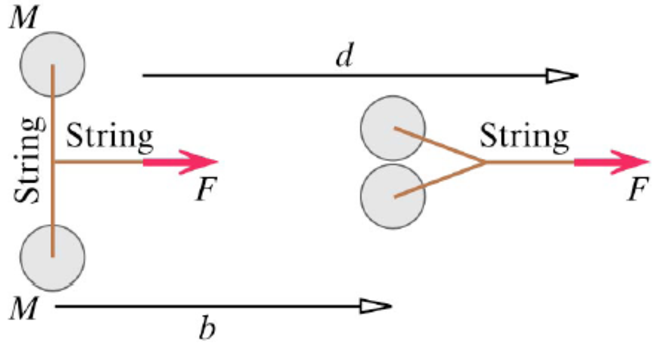
\includegraphics[width=0.6\textwidth]{figs/sliding_dumbells}

\item Santa Claus is skating on the magic ice near the North Pole, which is frictionless. A massless rope sticks out from the pole horizontally along a straight line. The rope's original length is $L_0$. Santa approaches the rope moving perpendicular to the direction of the rope and grabs the end of the rope. The diameter of the North Pole is $2a$. The rope then winds around the thin pole, $a<<L_0$, until Santa is half the original distance, $L_0/2$, from the pole. If Santa's original speed was $v_0$, what is his new speed? Assume there is no energy wasted in curving the rope around the pole. 

\item \label{Wcmproof}Prove that the work on the center of mass of a system of particles during a small time interval $\delta t$, which is defined by 
\[
\delta W_{\rm cm}\equiv \vec{F}_{\rm tot}\cdot \delta\vec{r}_{\rm cm},
\]
is equal to the change of the kinetic energy of the center of mass,
\[
T_{\rm cm}\equiv \frac{1}{2}M_{\rm tot}v_{\rm cm}^2, ~~~~~\delta T_{\rm cm}=M_{\rm tot}\vec{v}_{\rm cm}\cdot\delta\vec{v}_{\rm cm}.
\]
Use the following definitions:
\begin{eqnarray*}
\vec{F}_{\rm tot}&=&\sum_i \vec{F}_i,\\
M_{\rm tot}&=&\sum_i m_i,\\
\vec{r}_{cm}&=&\frac{1}{M_{\rm tot}}\sum_i m_i\vec{r}_i,\\
\vec{v}_{cm}&=&\frac{1}{M_{\rm tot}}\sum_i m_i\vec{v}_i.
\end{eqnarray*}

\end{enumerate} 

